%% no need for  \DeclareGraphicsExtensions{.pdf,.eps}

\documentclass[12pt,letterpaper,english]{article}
\usepackage{times}
\usepackage[T1]{fontenc}
\IfFileExists{url.sty}{\usepackage{url}}
                      {\newcommand{\url}{\texttt}}

\usepackage{babel}
%\usepackage{noweb}
\usepackage{Rd}

\usepackage{Sweave}

%\VignetteIndexEntry{Performance Attribution from Bacon}
%\VignetteDepends{PerformanceAnalytics}
%\VignetteKeywords{returns, performance, risk, benchmark, portfolio}
%\VignettePackage{PerformanceAnalytics}

%\documentclass[a4paper]{article}
%\usepackage[noae]{Sweave}
%\usepackage{ucs}
%\usepackage[utf8x]{inputenc}
%\usepackage{amsmath, amsthm, latexsym}
%\usepackage[top=3cm, bottom=3cm, left=2.5cm]{geometry}
%\usepackage{graphicx}
%\usepackage{graphicx, verbatim}
%\usepackage{ucs}
%\usepackage[utf8x]{inputenc}
%\usepackage{amsmath, amsthm, latexsym}
%\usepackage{graphicx}

\title{Stacked Bar Plot of Autocorrelation Coefficient}
\author{R Project for Statistical Computing}

\begin{document}
\Sconcordance{concordance:ACFbarplot.tex:ACFbarplot.Rnw:%
1 44 1 1 5 1 4 4 1 1 2 1 0 2 1 4 0 1 2 3 1}


\maketitle


\begin{abstract}
Creates an ACF chart stacked bar plot with the ACF and PACF set to some depict the ACF weightage of different lag factors.
\end{abstract}



\section{Usage}

In this example we use edhec database, to show autocorrelation effect of the return time series with respect to lag factors.

\begin{Schunk}
\begin{Sinput}
> library(PerformanceAnalytics)
> data(edhec)
> chart.Autocorrelation(edhec[,1:3])
\end{Sinput}
\end{Schunk}
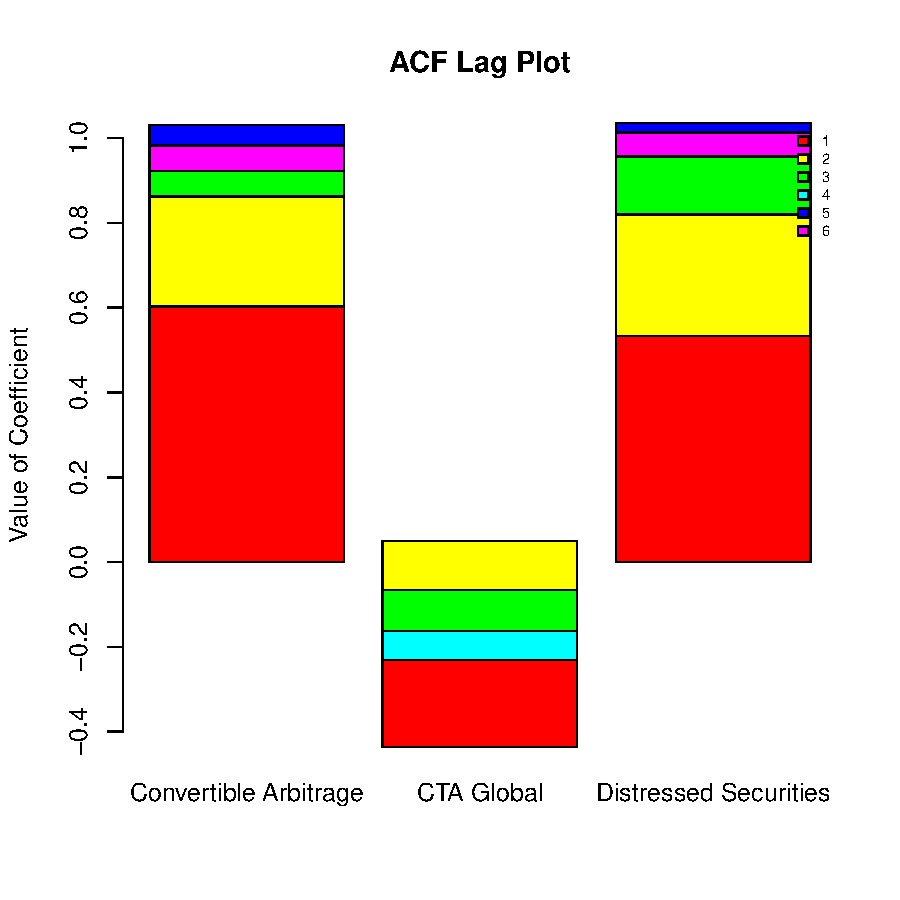
\includegraphics{ACFbarplot-003}



\end{document}
